\documentclass[conference]{IEEEtran}
\IEEEoverridecommandlockouts

\usepackage[T1]{fontenc}
\usepackage{amsmath,amssymb,amsthm}
\usepackage{booktabs}
\usepackage{graphicx}
\usepackage{cite}
\usepackage[hidelinks]{hyperref}

\newtheorem{proposition}{Proposition}
\newtheorem{definition}{Definition}

\begin{document}

\title{Fuzzy RFM Formal Concept Analysis for Customer Segmentation: Boundary-Aware, Describable and Stable Segments}

\author{\IEEEauthorblockN{Nandana Narayan Das}
\IEEEauthorblockA{ASAC, Alliance University\\Bengaluru, India\\nandanadas007@gmail.com}
\and
\IEEEauthorblockN{Tina Babu}
\IEEEauthorblockA{ASAC, Alliance University\\Bengaluru, India}
\and
\IEEEauthorblockN{Rekha R Nair}
\IEEEauthorblockA{ASAC, Alliance University\\Bengaluru, India}}

\maketitle

\begin{abstract}
RFM segmentation with formal concept analysis (FCA) gives explicitly described, hierarchically ordered segments, but its binary context puts customers on either side of a quintile cut point into disjoint segments although they behave almost identically. We replace the binary RFM context with a fuzzy one and build segments from Bělohlávek fuzzy concepts, adding a core-support threshold that removes the near-universal concepts the Łukasiewicz residuum otherwise makes frequent and a greedy concept summary with a $(1-1/e)$ guarantee. Crisp RFM-FCA is a special case of the method. On three retail datasets with rolling-origin out-of-sample evaluation and pre-registered analyses, fuzzy RFM-FCA predicts next-period purchase and spend better than crisp RFM-FCA (in 47 of 48 sensitivity settings), reaches more revenue in the top customer decile, and gives the most robust and stable segments among crisp FCA, K-means, Gaussian mixtures and fuzzy C-means. It is not a better predictor than log-RFM and is roughly level with fuzzy C-means, but its segments are exactly described by short rules and represent the 69--74\,\% of customers who lie near a quintile boundary.
\end{abstract}

\begin{IEEEkeywords}
Customer segmentation, RFM, formal concept analysis, fuzzy concept lattice, interpretability.
\end{IEEEkeywords}

\section{Introduction}

Recency, frequency and monetary value (RFM) are the most common basis for behavioural customer segmentation \cite{hughes1994,fader2005}. Each dimension is usually scored by quintile and customers are grouped by score combinations or by clustering \cite{chen2012,wedel2000}. Rungruang et al.\ \cite{rungruang2024} instead treat the fifteen quintile indicators (R1--R5, F1--F5, M1--M5) as a binary formal context and read segments off its concept lattice \cite{ganter1999}. Formal concepts are defined by their descriptions (e.g.\ $\{R5,F5,M5\}$), ordered in a hierarchy and linked by association rules, which makes them directly usable by marketers.

The binary context has a cost, named as future work in \cite{rungruang2024}: customers just below and just above a cut point receive disjoint attributes. This is common: 69--74\,\% of customers in our three datasets lie within 0.05 of a quintile cut point on some dimension. We make the context fuzzy and build segments from fuzzy formal concepts \cite{belohlavek2002,belohlavek2004}. Our contributions are: (i) a fuzzy RFM context whose 0.5-cut is the crisp context, a \emph{core-support} threshold and a greedy concept \emph{summary}; (ii) proofs that crisp RFM-FCA is a special case, that core support reduces to ordinary support, why sigma-count support fails under Łukasiewicz logic, and that the summary is within $1-1/e$ of optimal; and (iii) a replication of \cite{rungruang2024} and an out-of-sample comparison on three datasets against the crisp method, log-RFM and three clustering baselines, with analysis plans committed before each analysis.

\section{Related Work}

RFM summarises purchase history and is a sufficient input for lifetime-value projection under standard models \cite{fader2005}; segmentation commonly applies K-means to RFM \cite{chen2012}. Fuzzy RFM work softens the inputs or the assignment: Carrasco et al.\ \cite{carrasco2019} use 2-tuple fuzzy linguistic RFM scores before K-means, and Marín Díaz \cite{marindiaz2025} clusters RFM with fuzzy C-means \cite{bezdek1981} plus explainable-AI post-processing. In both, segments remain clusters without exact descriptions or order. FCA is widely used for knowledge discovery \cite{poelmans2013app,singh2016}; concept explosion is handled by support or stability pruning \cite{kuznetsov2007}, and rules are read along lattice covers \cite{luxenburger1991}. Fuzzy FCA generalises the incidence relation to a residuated lattice \cite{burusco1994,pollandt1997,belohlavek2002}; its surveys stress the much larger number of concepts \cite{poelmans2014,alwersh2022}. To our knowledge fuzzy concepts have not been used for RFM segmentation, and RFM-FCA has not been evaluated out of sample or against clustering on several datasets.

\section{Method}

\subsection{Crisp RFM-FCA}
For customers $G$, recency $R$, frequency $F$ (transaction lines) and monetary value $M$ are computed at a cutoff and mapped to mid-rank percentiles $u_d(g)\in(0,1]$, larger is better. The crisp score is $q_d = \lceil 5u_d\rceil$ and $(g,dk)\in I$ iff $q_d(g)=k$. Segments are concepts with support $\ge 0.04$ \cite{rungruang2024}.

\subsection{Fuzzy context and concepts}
With midpoints $c_k=(2k-1)/10$ and half-width $h=0.2$, term memberships are
\begin{equation}
\mu_k(u)=\max\bigl(0,\,1-|u-c_k|/h\bigr),
\end{equation}
with saturating outer shoulders; they form a Ruspini partition \cite{ruspini1969}. Memberships are rounded to $L=\{0,\tfrac12,1\}$, giving $\tilde I(g,dk)$. Over $L$ with a residuated implication $\to$ (Łukasiewicz $\min(1,1-a+b)$; Gödel as a check \cite{hajek1998}),
\begin{equation}
A^{\uparrow}(m)=\textstyle\bigwedge_{g}\bigl(A(g)\to\tilde I(g,m)\bigr),\quad
B^{\downarrow}(g)=\textstyle\bigwedge_{m}\bigl(B(m)\to\tilde I(g,m)\bigr),
\end{equation}
and fuzzy concepts are fixpoints $(A,B)$ \cite{belohlavek2004}; $B^{\downarrow}(g)$ is $g$'s membership degree. Intents are computed as the meet-closure of the generators $a\to\tilde I(g,\cdot)$.

\begin{definition}[Core support]
$\mathrm{cs}(B)=|\{g:B^{\downarrow}(g)=1\}|/|G|$. Fuzzy RFM-FCA keeps concepts with $\mathrm{cs}(B)\ge0.04$ and represents customers by their degrees in them.
\end{definition}

\subsection{Properties}
\begin{proposition}\label{prop:special}
(i) In the interior of quintile band $q$, $\mu_q>\tfrac12>\mu_k$ for $k\neq q$, so the 0.5-cut of $\tilde I$ is the crisp context. (ii) Over $\{0,1\}$ every residuated implication is classical, so fuzzy and crisp lattices, degrees and supports coincide.
\end{proposition}
\begin{proof}[Proof sketch]
(i) Interior points are $<0.1$ from $c_q$ and $>0.1$ from other midpoints. (ii) Residuation forces $a\to b=1$ iff $a\le b$.
\end{proof}

\begin{proposition}\label{prop:core}
For any residuated implication, $B^{\downarrow}(g)=1$ iff $B\le\tilde I(g,\cdot)$; hence core support is residuum-free, anti-monotone in $B$ (frequent intents form a down-set) and equal to support on binary data.
\end{proposition}

\begin{proposition}\label{prop:floor}
Under Łukasiewicz logic $B^{\downarrow}(g)\ge1-\max_m B(m)$, so every intent with all degrees $\le\tfrac12$ has sigma-count support $\ge\tfrac12$.
\end{proposition}

Proposition~\ref{prop:floor} explains why the naive extension fails: on Online Retail II, 2,649 of 3,841 Łukasiewicz concepts pass a sigma-count support of 0.04, dominated by intents such as $\{\tfrac12F1,\tfrac12F2,\tfrac12M1,\tfrac12M2\}$. Core support cuts them to 208.

\subsection{Summary view}
For communication we select $K$ segments maximising
\begin{equation}
f(S)=\textstyle\sum_{g}\max_{c\in S} w_c\,\mathbf{1}[B_c^{\downarrow}(g)=1],
\end{equation}
where $w_c=\sum_m B_c(m)$ is intent size; no outcome is used.

\begin{proposition}\label{prop:greedy}
$f$ is monotone submodular (a facility-location function), so greedy selection is within $1-1/e$ of the optimum \cite{nemhauser1978}.
\end{proposition}

All propositions are also verified numerically in the accompanying test suite.

\section{Experimental Design}

\textbf{Data.} Online Retail II \cite{chen2019uci} (1,067,371 lines; 5,878 customers; the base paper's dataset, used for replication and development), CDNOW \cite{fader2005} (69,659 purchases; 23,570 customers; 52--65\,\% buy once) and dunnhumby \emph{The Complete Journey} \cite{dunnhumby} (2.6M basket lines; 2,500 households).

\textbf{Protocol.} Rolling origin \cite{tashman2000} with four cutoffs per dataset; features from history, targets over the next 90 days: purchase (ROC AUC, logistic regression) and log spend ($R^2$, ridge). Within each cutoff, 5-fold cross-validation; rank scale, lattice, summary and clusters are fitted on training customers only. Regularisation is tuned by inner cross-validation. Differences are tested by a paired customer bootstrap pooled over cutoffs \cite{efron1993} with Holm correction \cite{holm1979}.

\textbf{Representations.} C-ctx / F-ctx: 15 crisp / fuzzy memberships (ablations); C-fca: crisp lattice \cite{rungruang2024}; F-fca-core: ours; log-RFM; K-means, Gaussian mixture (GMM) and fuzzy C-means (FCM, k-means++ seeding \cite{arthur2007}) on log-RFM. The base paper's silhouette rule \cite{rousseeuw1987} chose $k=2$ in all 60 folds, so we report $k=10$.

\textbf{Pre-registration.} An analysis plan and eleven addenda were committed to the repository before each analysis. The method was developed on Online Retail II; CDNOW and dunnhumby served as confirmation with the method unchanged.

\section{Results}

\begin{table*}[t]
\centering\footnotesize
\caption{Out-of-sample prediction of the next 90 days (means over four cutoffs; regularisation tuned by inner cross-validation). Best value per column in bold.}
\label{tab:prediction}
\begin{tabular}{lcccccc}
\toprule
 & \multicolumn{3}{c}{ROC AUC (purchase)} & \multicolumn{3}{c}{$R^2$ (log spend)} \\
\cmidrule(lr){2-4}\cmidrule(lr){5-7}
Representation & Retail II & CDNOW & dunnhumby & Retail II & CDNOW & dunnhumby \\
\midrule
C-ctx & 0.782 & 0.784 & 0.869 & 0.296 & 0.209 & 0.511 \\
C-fca (base) & 0.780 & 0.784 & 0.855 & 0.299 & 0.222 & 0.508 \\
F-ctx & \textbf{0.787} & \textbf{0.789} & 0.877 & 0.304 & 0.219 & \textbf{0.525} \\
F-fca-core (ours) & 0.786 & 0.788 & 0.865 & \textbf{0.308} & 0.235 & 0.517 \\
log-RFM & 0.786 & 0.788 & \textbf{0.887} & 0.293 & \textbf{0.241} & 0.517 \\
K-means, $k{=}10$ & 0.764 & 0.777 & 0.828 & 0.289 & 0.236 & 0.498 \\
GMM, $k{=}10$ & 0.770 & 0.778 & 0.875 & 0.260 & 0.232 & 0.453 \\
FCM, $k{=}10$ & 0.783 & 0.786 & 0.860 & 0.290 & 0.239 & 0.511 \\
\bottomrule
\end{tabular}
\end{table*}

\begin{table*}[t]
\centering\footnotesize
\caption{Paired differences (first minus second representation), tuned regularisation, pooled over four cutoffs. $^{*}$: 95\,\% customer-bootstrap interval excludes zero.}
\label{tab:comparisons}
\begin{tabular}{lcccccc}
\toprule
 & \multicolumn{3}{c}{$\Delta$ AUC} & \multicolumn{3}{c}{$\Delta R^2$} \\
\cmidrule(lr){2-4}\cmidrule(lr){5-7}
Comparison & Retail II & CDNOW & dunnhumby & Retail II & CDNOW & dunnhumby \\
\midrule
Fuzzification (memberships) & +0.0048$^{*}$ & +0.0048$^{*}$ & +0.0076$^{*}$ & +0.0080$^{*}$ & +0.0099$^{*}$ & +0.0141$^{*}$ \\
Fuzzy vs crisp RFM-FCA & +0.0063$^{*}$ & +0.0040$^{*}$ & +0.0098$^{*}$ & +0.0089$^{*}$ & +0.0124$^{*}$ & +0.0089$^{*}$ \\
Lattice beyond memberships & -0.0008 & -0.0007 & -0.0117$^{*}$ & +0.0044$^{*}$ & +0.0154$^{*}$ & -0.0082$^{*}$ \\
vs K-means, $k{=}10$ & +0.0220$^{*}$ & +0.0111$^{*}$ & +0.0372$^{*}$ & +0.0189$^{*}$ & -0.0017 & +0.0186$^{*}$ \\
vs GMM, $k{=}10$ & +0.0163$^{*}$ & +0.0102$^{*}$ & -0.0101$^{*}$ & +0.0487$^{*}$ & +0.0024 & +0.0634$^{*}$ \\
vs FCM, $k{=}10$ & +0.0029$^{*}$ & +0.0021$^{*}$ & +0.0052 & +0.0180$^{*}$ & -0.0047$^{*}$ & +0.0058 \\
\bottomrule
\end{tabular}
\end{table*}


\textbf{Replication.} Our crisp RFM-FCA reproduces \cite{rungruang2024}: 805,620 lines, 5,878 customers and 208 concepts; published concept sizes are matched to within 0.8 customers on average and all 18 rules within 0.01 confidence.

\textbf{Development and confirmation.} The first specification, with sigma-count support, failed as Proposition~\ref{prop:floor} predicts (AUC 0.733 vs 0.781 for crisp); core support fixed it. On CDNOW all seven pre-registered claims replicated; on dunnhumby four did (fuzzy memberships and lattice beat their crisp counterparts), while the lattice adding spend signal beyond the fuzzy memberships and the robustness claims did not. We therefore do not claim the latter two.

\textbf{Prediction} (Tables~\ref{tab:prediction}, \ref{tab:comparisons}). On all three datasets, fuzzy memberships beat crisp scores (0.005--0.008 AUC, 0.008--0.014 $R^2$) and fuzzy RFM-FCA beats crisp RFM-FCA (0.004--0.010 AUC, 0.009--0.012 $R^2$). It beats K-means ($k=10$) in five of six cells and GMM in four, and is roughly level with FCM. With $k=2$ every clustering baseline trails by 0.018--0.181 AUC. No segmentation beats log-RFM overall, which keeps the exact values; adding fuzzy concept degrees to log-RFM still raises spend $R^2$ by 0.020 (Online Retail II) and 0.015 (CDNOW).

\begin{table*}[t]
\centering\footnotesize
\caption{Share of next-90-day revenue (\%) held by the top 10\,\% and 20\,\% of customers ranked by predicted spend (means over four cutoffs).}
\label{tab:targeting}
\begin{tabular}{lcccccc}
\toprule
 & \multicolumn{3}{c}{Top 10\,\%} & \multicolumn{3}{c}{Top 20\,\%} \\
\cmidrule(lr){2-4}\cmidrule(lr){5-7}
Representation & Retail II & CDNOW & dunnhumby & Retail II & CDNOW & dunnhumby \\
\midrule
C-fca (base) & 52.6 & 52.6 & 28.3 & 71.6 & 70.6 & 50.1 \\
F-fca-core (ours) & 55.4 & 53.5 & 30.5 & 71.8 & 70.4 & 50.7 \\
F-ctx & 55.6 & 52.8 & 30.6 & 73.4 & 70.1 & 50.9 \\
log-RFM & 58.0 & 52.8 & 31.2 & 72.3 & 69.9 & 50.0 \\
K-means, $k{=}10$ & 54.1 & 51.6 & 28.6 & 70.3 & 68.7 & 48.3 \\
GMM, $k{=}10$ & 51.2 & 51.2 & 21.7 & 70.1 & 68.0 & 38.7 \\
FCM, $k{=}10$ & 36.2 & 53.8 & 26.8 & 71.2 & 70.2 & 49.5 \\
\bottomrule
\end{tabular}
\end{table*}


\textbf{Targeting} (Table~\ref{tab:targeting}). Ranking by fuzzy RFM-FCA reaches 0.9--2.9 percentage points more of next-period revenue in the top decile than crisp RFM-FCA on every dataset ($p\le0.01$), and more than K-means and GMM at both depths. FCM is mostly level but fails on the Online Retail II top decile (36.2\,\% vs 55.4\,\%).

\begin{table*}[t]
\centering\footnotesize
\caption{Structural agreement (correlation of customer-pair similarities between a reference fit and a perturbed fit; 1 = identical), mean over 20 replicates. Robustness: 5\,\% of invoices dropped. Stability: bootstrap resample of customers.}
\label{tab:structure}
\begin{tabular}{lcccccc}
\toprule
 & \multicolumn{3}{c}{Robustness} & \multicolumn{3}{c}{Stability} \\
\cmidrule(lr){2-4}\cmidrule(lr){5-7}
Representation & Retail II & CDNOW & dunnhumby & Retail II & CDNOW & dunnhumby \\
\midrule
C-fca (base) & 0.886 & 0.936 & 0.928 & 0.957 & 0.987 & 0.936 \\
F-fca-core (ours) & 0.958 & 0.955 & 0.948 & 0.986 & 0.993 & 0.972 \\
K-means, $k{=}10$ & 0.760 & 0.907 & 0.650 & 0.683 & 0.937 & 0.692 \\
GMM, $k{=}10$ & 0.858 & 0.816 & 0.878 & 0.818 & 0.904 & 0.843 \\
FCM, $k{=}10$ & 0.913 & 0.929 & 0.942 & 0.944 & 0.966 & 0.914 \\
\bottomrule
\end{tabular}
\end{table*}


\textbf{Robustness and stability} (Table~\ref{tab:structure}). Agreement is the correlation of 20,000 customer-pair similarities between a reference and a perturbed fit (5\,\% of invoices dropped, or customers bootstrapped; 20 replicates). Fuzzy RFM-FCA has the highest mean on every dataset, beats crisp RFM-FCA in all robustness replicates and K-means and GMM in essentially all; against FCM the margin is small, but its worst case is better in all six cells.

\begin{table*}[t]
\centering\footnotesize
\caption{Structural interpretability proxies on the full data (Retail II / CDNOW / dunnhumby). Fidelity: F1 between ``satisfies the segment's R/F/M description'' and ``is a member''. Conditions: constrained dimensions per description.}
\label{tab:interpretability}
\begin{tabular}{lcccc}
\toprule
Representation & Segments & Fidelity (F1) & Conditions & Segments per customer \\
\midrule
C-fca (base) & 51 / 54 / 49 & 1.00 / 1.00 / 1.00 & 1.5 / 1.6 / 1.5 & 5.3 / 6.2 / 5.5 \\
F-fca-core (ours) & 208 / 238 / 215 & 1.00 / 1.00 / 1.00 & 1.8 / 1.9 / 1.8 & 19.5 / 24.0 / 20.9 \\
K-means, $k{=}10$ & 10 / 10 / 10 & 0.68 / 0.74 / 0.74 & 3.0 / 3.0 / 3.0 & 1.0 / 1.0 / 1.0 \\
GMM, $k{=}10$ & 10 / 10 / 10 & 0.53 / 0.80 / 0.67 & 3.0 / 3.0 / 3.0 & 1.0 / 1.0 / 1.0 \\
FCM, $k{=}10$ & 10 / 10 / 10 & 0.66 / 0.71 / 0.73 & 3.0 / 3.0 / 3.0 & 1.0 / 1.0 / 1.0 \\
\bottomrule
\end{tabular}
\end{table*}


\textbf{Interpretability} (Table~\ref{tab:interpretability}). FCA segments are exactly described by their intents in fewer than two conditions, whereas the tightest R/F/M description of a cluster disagrees with its membership for 20--47\,\% of customers. The cost is about four times as many segments as crisp FCA, and mean rule confidence is slightly lower (e.g.\ 0.71 vs 0.73), although individual rules sharpen: $\{R5,M5\}\Rightarrow\{R5,F5,M5\}$ has confidence 0.81 crisp, while $\{R5,M5\}\Rightarrow\{R5,\tfrac12F5,M5\}$ has 0.92. The 10-concept greedy summary leaves each customer in one or two segments; on Online Retail II it includes $\{F5,M5\}$ (10.3\,\% of customers, 55.3\,\% of spend) and $\{R5,F5,M5\}$ (4.8\,\%, 36.9\,\%). It beats the 10-concept crisp summary on all datasets (AUC $+0.005$ to $+0.026$) and is far more stable, but predicts worse than FCM with ten clusters (AUC $-0.005$ to $-0.047$).

\begin{table}[t]
\centering\footnotesize
\caption{Sensitivity analysis: number of setting $\times$ dataset $\times$ metric cells in which the fuzzy variant is significantly better (95\,\% interval above zero) and significantly worse. Settings: support 0.02/0.04/0.06, membership half-width 0.15/0.20/0.25, horizon 60/90/180 days.}
\label{tab:sensitivity}
\begin{tabular}{p{3.3cm}cc}
\toprule
Comparison & Fuzzy significantly better & Significantly worse \\
\midrule
Fuzzy vs crisp RFM-FCA & 47 / 48 & 0 \\
Fuzzy vs crisp memberships & 29 / 30 & 1 \\
Fuzzy vs crisp summary ($K = 5, 10, 20, 30$) & 18 / 24 & 1 \\
\bottomrule
\end{tabular}
\end{table}


\begin{figure*}[t]
\centering
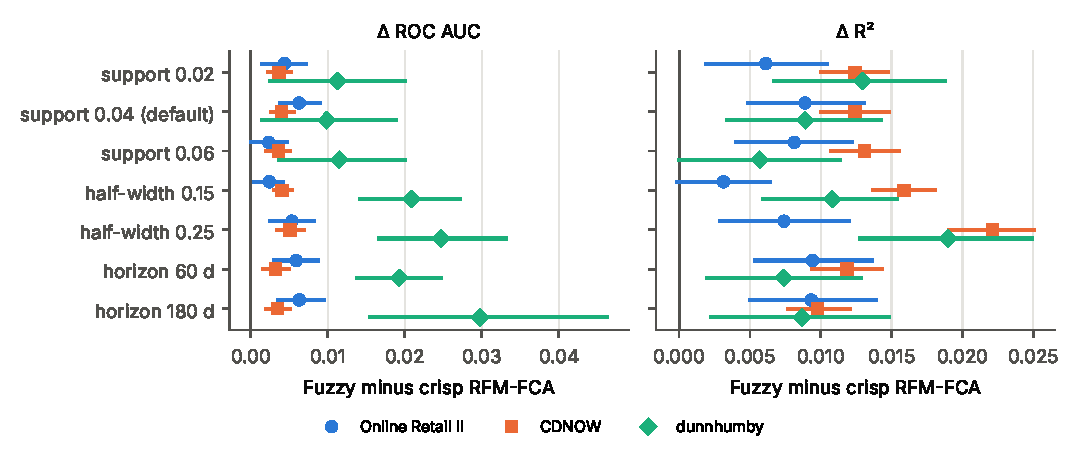
\includegraphics[width=0.82\textwidth]{figures/sensitivity.pdf}
\caption{Fuzzy minus crisp RFM-FCA under one-at-a-time parameter changes, with 95\,\% bootstrap intervals.}
\label{fig:sens}
\end{figure*}

\textbf{Sensitivity} (Table~\ref{tab:sensitivity}, Fig.~\ref{fig:sens}). Varying the support threshold (0.02--0.06, i.e.\ about 140--500 fuzzy segments), membership width (0.15--0.25) and horizon (60--180 days), fuzzy RFM-FCA beats crisp RFM-FCA significantly in 47 of 48 cells and is never worse.

\section{Discussion and Conclusion}

Fuzzifying the RFM context consistently improves on crisp quintiles, both as attributes and as concept lattices, on three datasets and across all parameter settings, with the gain concentrated in the most valuable decile, and it yields the most stable segment structure of the methods compared. The limits are equally clear: segments compress the data, so log-RFM is at least as accurate for pure prediction; most of the predictive gain comes from the fuzzy memberships rather than the lattice; accuracy is roughly level with fuzzy C-means; and the full lattice has about four times as many segments as the crisp one. We therefore recommend the full fuzzy lattice for modelling and targeting and the 10-concept summary for communicating segments. Limitations: effect sizes are small (0.004--0.010 AUC), interpretability was measured by structural proxies rather than with marketers, the later analyses reuse the same three datasets, and only retail data and a three-level truth scale were studied.

\section*{Data and Code Availability}
Online Retail II and CDNOW are public; dunnhumby data are available from the provider. Code, analysis plans and aggregate results: \url{https://github.com/nandana-das/rfm-fuzzy}.

\bibliographystyle{IEEEtran}
\bibliography{refs}

\end{document}
